% Provenance (never printed): 6e geography and cycle 3 sciences (locating a
% place on the globe: parallels, meridians, latitude, longitude; the Earth's
% rotation and time zones); see sources/book1/PROVENANCE.md.
% Book 1, grade 6, chapter 2.
\chapter{纬度、经度与时区}\label{ch:g6:latitude-longitude}

夜幕降临在大海上。一艘帆船的甲板上，
1750 年，航海家举起仪器对准一颗明亮的恒星，
测量它在海面上方的高度。只需几分钟的计算，他便知道
船在\omterm{def:g3:continents-and-oceans:equator}{赤道}以北多少度。但船在东西方向上的位置呢？他无从得知。
这个问题十分严重，1714 年英国议会
曾许下巨额奖金，奖给能在海上测定这一位置的人。
如今，你口袋里的手机只需一秒，就能给出这两个答案。
% ledger: rmg:15deg-per-hour, rmg:longitude-act-1714

\begin{omfigure}

\includegraphics[width=0.62\linewidth]{images/book1/ai/g6-navigator-sextant.jpg}

{\small 十八世纪的航海家测量海平线上方一颗恒星的高度。
（AI 插图。）}
\end{omfigure}

\begin{recall}
\omterm{def:g3:continents-and-oceans:globe}{地球仪}是地球的小模型。\omterm{def:g3:continents-and-oceans:equator}{赤道}是绕\omterm{def:g3:continents-and-oceans:globe}{地球仪}中部、
位于\omterm{def:g3:continents-and-oceans:poles}{北极}和\omterm{def:g3:continents-and-oceans:poles}{南极}正中间的一条线，
它把地球分为\omterm{def:g3:continents-and-oceans:equator}{北半球}和\omterm{def:g3:continents-and-oceans:equator}{南半球}
（见\cref{ch:g3:continents-and-oceans}）。物理课本中已经说明，
地球绕着穿过两极的地轴自转，
每天一圈，这种自转带来了昼夜交替。
\end{recall}

\section{纬线与纬度}

要说明某地在地球上的位置，需要两个数字，
就像电影院里座位的排号和列号。第一个数字
表示该地位于\omterm{def:g3:continents-and-oceans:equator}{赤道}以北或以南多远。

想象把地球通过两极切成两半，就像从果柄向下切开
一个苹果。切面上（左下图），\omterm{def:g3:continents-and-oceans:equator}{赤道}是穿过中心的水平线。
地表上的地点 P 从地心望去，
位于该线上方或下方某一角度处，这个角度
就是它的\omterm{def:g6:latitude-longitude:latitude}{纬度}。

\begin{omfigure}
\begin{minipage}[t]{0.48\linewidth}\centering
\begin{tikzpicture}[scale=0.95]
  \def\R{2.2}
  \fill[blue!6] (0,0) circle (\R);
  \draw[thick] (0,0) circle (\R);
  % parallels seen edge-on: horizontal chords
  \foreach \a in {-60,-30,30,60}{
    \draw[blue!45, densely dashed] ({-\R*cos(\a)},{\R*sin(\a)}) -- ({\R*cos(\a)},{\R*sin(\a)});}
    \draw[green!50!black, thick] (-\R,0) -- (\R,0);
  \node[font=\scriptsize, green!50!black, anchor=west] at (\R,0) {赤道，$0^\circ$};
  \draw[blue!60!black, thick] ({-\R*cos(40)},{\R*sin(40)}) -- ({\R*cos(40)},{\R*sin(40)});
  \draw[->, thick] (0,0) -- ({\R*cos(40)},{\R*sin(40)});
  \fill (0,0) circle (1.4pt) node[below left, font=\scriptsize, inner sep=1pt] {球心};
  \fill ({\R*cos(40)},{\R*sin(40)}) circle (1.6pt)
    node[above right, font=\scriptsize\bfseries, inner sep=1pt] {P};
  \draw[red!70!black, thick] (0.9,0) arc (0:40:0.9);
  \node[red!70!black, font=\scriptsize] at (20:1.25) {$40^\circ$};
  \node[font=\scriptsize, blue!60!black, anchor=east] at ({-\R*cos(40)},{\R*sin(40)}) {纬线 $40^\circ$\,北};
  \fill (0,\R) circle (1.4pt) node[above, font=\scriptsize] {北极，$90^\circ$\,北};
  \fill (0,-\R) circle (1.4pt) node[below, font=\scriptsize] {南极，$90^\circ$\,南};
\end{tikzpicture}

{\small \omterm{def:g6:latitude-longitude:latitude}{纬度}：在地心处度量的，\omterm{def:g3:continents-and-oceans:equator}{赤道}与该地之间的
夹角。}
\end{minipage}\hfill
\begin{minipage}[t]{0.48\linewidth}\centering
\begin{tikzpicture}[scale=0.95]
  \def\R{2.2}
  \fill[green!6] (0,0) circle (\R);
  \draw[thick] (0,0) circle (\R);
  \foreach \a in {0,30,...,330}{\draw[black!25] (0,0) -- (\a:\R);}
    \draw[red!70!black, very thick] (0,0) -- (270:\R)
    node[below, font=\scriptsize, align=center] {本初子午线 \\（格林尼治），$0^\circ$};
  \draw[blue!60!black, very thick] (0,0) -- (330:\R)
    node[right, font=\scriptsize] {$60^\circ$\,东};
  \draw[black!60, thick] (0,0) -- (210:\R) node[left, font=\scriptsize] {$60^\circ$\,西};
  \draw[black!60, thick] (0,0) -- (90:\R) node[above, font=\scriptsize] {$180^\circ$};
  \draw[red!70!black, thick] (270:0.9) arc (270:330:0.9);
  \node[red!70!black, font=\scriptsize] at (300:1.25) {$60^\circ$};
    \fill (0,0) circle (1.6pt) node[above left, font=\scriptsize, inner sep=1.5pt, fill=green!6] {北极};
  \draw[->, thick, black!70] (40:2.55) arc (40:80:2.55);
  \node[font=\scriptsize, black!70, anchor=south west] at (55:2.6) {地球自转};
  \node[font=\scriptsize, anchor=west] at (2.0,-1.6) {向东 $\circlearrowleft$};
\end{tikzpicture}

{\small \omterm{def:g6:latitude-longitude:longitude}{经度}：从\omterm{def:g3:continents-and-oceans:poles}{北极}上方看到的地球。角度从
\omterm{def:g6:latitude-longitude:longitude}{本初子午线}起算，向东或向西量取。}
\end{minipage}
% ledger: rmg:latitude-def, rmg:longitude-def
\end{omfigure}

\begin{definition}[纬线与纬度]\label{def:g6:latitude-longitude:latitude}
称\emph{纬线}\index{纬线}为绕地球画出的、与\omterm{def:g3:continents-and-oceans:equator}{赤道}平行的
圆；同一纬线上的各地到\omterm{def:g3:continents-and-oceans:equator}{赤道}的距离都相等。
某地的\emph{纬度}\index{纬度}是在地心处度量的角度，
即\omterm{def:g3:continents-and-oceans:equator}{赤道}与该地之间的夹角。纬度从\omterm{def:g3:continents-and-oceans:equator}{赤道}处的
$0^\circ$ 增至两极处的 $90^\circ$，并说明该地位于
\omterm{def:g3:continents-and-oceans:equator}{赤道}以北（N）还是以南（S）。
% ledger: rmg:latitude-def
\end{definition}

\omterm{def:g3:continents-and-oceans:equator}{赤道}本身也是一条\omterm{def:g6:latitude-longitude:latitude}{纬线}，是其中最长的一条，\omterm{def:g6:latitude-longitude:latitude}{纬度}为 $0^\circ$。
\omterm{def:g6:latitude-longitude:latitude}{纬线}越靠近两极越短，每个极点都只是
一个点，位于北纬 $90^\circ$ 或南纬 $90^\circ$。沿着从极点到
\omterm{def:g3:continents-and-oceans:equator}{赤道}的一条线，每一度\omterm{def:g6:latitude-longitude:latitude}{纬度}约为 \qty{111}{km}。
% ledger: rmg:latitude-def

\omterm{def:g6:latitude-longitude:latitude}{纬度}是最容易确定的数：它可以从天空中求得。白天，
水手在正午测量太阳的高度；夜晚，在\omterm{def:g3:continents-and-oceans:equator}{北半球}，
他们测量\omterm{def:g3:continents-and-oceans:poles}{北极}星的高度。开篇图中的
领航员正是在做这件事。
% ledger: rmg:15deg-per-hour

\omterm{def:g3:continents-and-oceans:poles}{北极}星几乎恰好位于地轴的延长线上，
向\omterm{def:g3:continents-and-oceans:poles}{北极}之外延伸，离地球非常遥远，其光线以平行线的方式到达
地球上的每一个地方。在\omterm{def:g3:continents-and-oceans:poles}{北极}，它
位于正上方，与地平线成 $90^\circ$ 角；在\omterm{def:g3:continents-and-oceans:equator}{赤道}，它位于
北方地平线上，高度为 $0^\circ$。两者之间的规律很简单：
\emph{\omterm{def:g3:continents-and-oceans:poles}{北极}星在北方地平线以上的高度，以角度计，
等于\omterm{def:g6:latitude-longitude:latitude}{纬度}}。下图说明了这两个
角为何相等。
% ledger: nsta:polaris-latitude

\begin{omfigure}
\begin{tikzpicture}[scale=1.1, font=\scriptsize]
  \def\R{1.7}
  \coordinate (O) at (0,0);
  \coordinate (P) at ({\R*cos(40)},{\R*sin(40)});
  \fill[blue!8] (O) circle (\R);
  \draw[black!70] (O) circle (\R);
  % equator and axis
  \draw[black!50] (-\R,0) -- (\R,0);
  \node[black!60, anchor=north east] at (-0.15,0) {赤道};
  \draw[black!70, -{Stealth[length=2mm]}] (0,-\R-0.3) -- (0,\R+1.7);
  \node[anchor=east, align=right] at (-0.1,\R+1.45) {指向北极星 \\（非常遥远）};
  \node[anchor=south east] at (0,\R) {北};
  % radius to P and latitude angle at the centre
  \draw[black!80] (O) -- (P);
  \draw[red!70!black, thick] (0.55,0) arc (0:40:0.55);
  \node[red!70!black] at (20:0.8) {$40^\circ$};
  % horizon at P (tangent) and the ray to the Pole Star (parallel to the axis)
  \draw[black!70, thick] ($(P)+({-sin(40)*1.5},{cos(40)*1.5})$) -- ($(P)+({sin(40)*1.6},{-cos(40)*1.6})$);
  \node[anchor=south, rotate=-50, inner sep=2pt] at ($(P)+({sin(40)*1.15},{-cos(40)*1.15})$) {地平线};
  \draw[orange!80!black, thick, -{Stealth[length=2mm]}] (P) -- ++(0,1.45);
  \draw[red!70!black, thick] ($(P)+(0,0.7)$) arc (90:130:0.7);
  \node[red!70!black] at ($(P)+(110:0.98)$) {$40^\circ$};
  \fill (P) circle (1.4pt);
  \node[anchor=west] at ($(P)+(0.3,0.05)$) {观察者位于北纬 $40^\circ$};
\end{tikzpicture}

{\small 为何\omterm{def:g3:continents-and-oceans:poles}{北极}星的高度等于\omterm{def:g6:latitude-longitude:latitude}{纬度}（示意图，
不按比例）。\omterm{def:g3:continents-and-oceans:poles}{北极}星的光线平行于地轴射来
（橙色）。观察者的地平线与过观察者的半径垂直；
地轴与\omterm{def:g3:continents-and-oceans:equator}{赤道}垂直。因此，地平线与\omterm{def:g3:continents-and-oceans:poles}{北极}星的
方向之间的夹角与\omterm{def:g6:latitude-longitude:latitude}{纬度}相等，即
地心处\omterm{def:g3:continents-and-oceans:equator}{赤道}与观察者之间的夹角。}
% ledger: nsta:polaris-latitude
\end{omfigure}

\begin{example}[夜间的领航员]\label{ex:g6:latitude-longitude:pole-star}
一名领航员测得\omterm{def:g3:continents-and-oceans:poles}{北极}星位于北方
地平线以上 $41^\circ$ 处。此船位于北纬 $41^\circ$，大约在\omterm{def:g3:continents-and-oceans:equator}{赤道}以北 $41 \times 111
\approx \num{4550}$~千米处。领航员向北航行时，发现
星每晚都略高一些；向南驶向\omterm{def:g3:continents-and-oceans:equator}{赤道}时，它
逐渐降向地平线。\omterm{def:g3:continents-and-oceans:equator}{赤道}以南无法看到\omterm{def:g3:continents-and-oceans:poles}{北极}星，
因为它始终位于地平线以下：在那里，正午的太阳可给出
\omterm{def:g6:latitude-longitude:latitude}{纬度}。
\end{example}
% ledger: nsta:polaris-latitude, rmg:latitude-def, rmg:15deg-per-hour

\section{经线与经度}

第二个数字说明某地位于东侧还是西侧，
但没有像\omterm{def:g3:continents-and-oceans:equator}{赤道}那样天然的起始线，必须人为选定。

\begin{definition}[经线、经度与本初子午线]\label{def:g6:latitude-longitude:longitude}
\emph{经线}\index{经线}是\omterm{def:g3:continents-and-oceans:globe}{地球仪}上从\omterm{def:g3:continents-and-oceans:poles}{北极}到
\omterm{def:g3:continents-and-oceans:poles}{南极}画出的半圆。被选为起点的那条经线称为\emph{本初子午线}\index{本初子午线}，
即穿过伦敦格林尼治旧皇家天文台的
那条经线。某地的
\emph{经度}\index{经度}是从地轴看去，本初子午线与
该地所在经线之间的夹角。它从本初子午线处的 $0^\circ$
增至 $180^\circ$，并说明该地位于本初子午线的
东（E）侧还是西（W）侧。
% ledger: rmg:longitude-def
\end{definition}

所有\omterm{def:g6:latitude-longitude:longitude}{经线}都交于两极，且长度都相等。在
地球上与格林尼治相对的一侧，东经 $180^\circ$ \omterm{def:g6:latitude-longitude:longitude}{经线}与
西经 $180^\circ$ \omterm{def:g6:latitude-longitude:longitude}{经线}是同一条线。

\begin{omfigure}
\begin{minipage}[c]{0.46\linewidth}\centering
\begin{tikzpicture}
  \begin{axis}[axis equal image, hide axis, width=\linewidth,
      xmin=-1.05, xmax=1.05, ymin=-1.05, ymax=1.12, clip=false]
    \fill[omSea] (axis cs:0,0) circle (1);
    \addplot[fill=omLithAlluv, draw=black!45, line width=0.2pt] table {figdata/out/grade-6-graticule-land.dat};
    \addplot[blue!50!black, line width=0.35pt] table {figdata/out/grade-6-graticule-parallels.dat};
    \addplot[black!55, line width=0.35pt] table {figdata/out/grade-6-graticule-meridians.dat};
        \addplot[green!50!black, line width=1.1pt] table {figdata/out/grade-6-graticule-equator.dat};
    \addplot[red!70!black, line width=1.1pt] table {figdata/out/grade-6-graticule-prime.dat};
    \draw[black!70] (axis cs:0,0) circle (1);
    \fill (axis cs:0,0.9063) circle (1.3pt);
        \node[font=\scriptsize, above left, inner sep=1.5pt] at (axis cs:0,0.9063) {北};
  \end{axis}
\end{tikzpicture}
\end{minipage}\hfill
\begin{minipage}[c]{0.5\linewidth}
{\small \omterm{def:g3:continents-and-oceans:globe}{地球仪}，\omterm{def:g6:latitude-longitude:latitude}{纬线}（蓝色）与\omterm{def:g6:latitude-longitude:longitude}{经线}（灰色）每隔
$30^\circ$ 画出一条。\omterm{def:g3:continents-and-oceans:equator}{赤道}以粗绿线画出，\omterm{def:g6:latitude-longitude:longitude}{本初子午线}以
红色表示；二者在加纳以南的\omterm{def:g2:water-on-earth:ocean}{海洋}中相交，\omterm{def:g6:latitude-longitude:latitude}{纬度} $0^\circ$，
\omterm{def:g6:latitude-longitude:longitude}{经度} $0^\circ$。每条\omterm{def:g6:latitude-longitude:longitude}{经线}都从一极延伸到另一极；每条\omterm{def:g6:latitude-longitude:latitude}{纬线}
都是围绕地轴的圆。（陆地数据：Natural Earth。）}
% ledger: data:ne-land (figdata/grade-6/graticule.py)
\end{minipage}
\end{omfigure}

\begin{history}[选择本初子午线]
长期以来，各国绘制\omterm{def:g2:drawing-to-map:map}{地图}时都采用各自的起始\omterm{def:g6:latitude-longitude:longitude}{经线}：
伦敦、巴黎等地都曾被采用。1884 年 10 月，多国代表
齐聚华盛顿，商定全球统一的一条\omterm{def:g6:latitude-longitude:longitude}{经线}。
10 月 13 日，与会代表投票，提议以
经过格林尼治天文台的\omterm{def:g6:latitude-longitude:longitude}{经线}为\omterm{def:g6:latitude-longitude:longitude}{本初子午线}：21 国投赞成票，1 国投反对票，
2 国弃权。
% ledger: rmg:longitude-def, meridian:1884-vote
\end{history}

\section{用两个角度确定地点}

由\omterm{def:g6:latitude-longitude:latitude}{纬度}和\omterm{def:g6:latitude-longitude:longitude}{经度}可以确定地球上的任一地点，
在\omterm{def:g2:drawing-to-map:map}{地图}或\omterm{def:g3:continents-and-oceans:globe}{地球仪}上均可找到。书写时先写\omterm{def:g6:latitude-longitude:latitude}{纬度}：例如开罗位于
约 $30^\circ$\,N，$31^\circ$\,E。
% ledger: data:b1-ne-places (figdata/grade-6/cities.py)

\begin{omfigure}
\begin{tikzpicture}
  \begin{axis}[ommap, width=\linewidth,
      xtick={-180,-150,...,180}, ytick={-90,-60,...,90},
      xticklabels={$180^\circ$,$150^\circ$西,$120^\circ$西,$90^\circ$西,$60^\circ$西,$30^\circ$西,$0^\circ$,
                   $30^\circ$东,$60^\circ$东,$90^\circ$东,$120^\circ$东,$150^\circ$东,$180^\circ$},
      yticklabels={$90^\circ$南, $60^\circ$南, $30^\circ$南, $0^\circ$,$30^\circ$北, $60^\circ$北, $90^\circ$北},
      tick label style={font=\tiny}, grid style={black!35, line width=0.3pt}]
    \addplot[fill=omLithAlluv, draw=black!45, line width=0.2pt] table {figdata/out/shared-geo-land.dat};
        \draw[green!50!black, line width=0.9pt] (axis cs:-180,0) -- (axis cs:180,0);
    \draw[red!70!black, line width=0.9pt] (axis cs:0,-90) -- (axis cs:0,90);
    \addplot[only marks, mark=*, mark size=1.2pt, black, point meta=explicit symbolic, visualization depends on={value \thisrow{anchor}\as\anc}]
      table[x=lon, y=lat, meta=name] {figdata/out/grade-6-cities-map.dat};
    \node[black, font=\tiny, inner sep=1.2pt, fill=white, fill opacity=0.75, text opacity=1, anchor=south] at (axis cs:-21.936,64.144) {雷克雅未克};
    \node[black, font=\tiny, inner sep=1.2pt, fill=white, fill opacity=0.75, text opacity=1, anchor=south] at (axis cs:-0.119,51.502) {伦敦};
    \node[black, font=\tiny, inner sep=1.2pt, fill=white, fill opacity=0.75, text opacity=1, anchor=west] at (axis cs:-73.996,40.722) {纽约};
    \node[black, font=\tiny, inner sep=1.2pt, fill=white, fill opacity=0.75, text opacity=1, anchor=east] at (axis cs:-118.232,34.049) {洛杉矶};
    \node[black, font=\tiny, inner sep=1.2pt, fill=white, fill opacity=0.75, text opacity=1, anchor=east] at (axis cs:-78.502,-0.213) {基多};
    \node[black, font=\tiny, inner sep=1.2pt, fill=white, fill opacity=0.75, text opacity=1, anchor=west] at (axis cs:-43.212,-22.907) {里约热内卢};
    \node[black, font=\tiny, inner sep=1.2pt, fill=white, fill opacity=0.75, text opacity=1, anchor=north] at (axis cs:18.433,-33.918) {开普敦};
    \node[black, font=\tiny, inner sep=1.2pt, fill=white, fill opacity=0.75, text opacity=1, anchor=west] at (axis cs:36.815,-1.281) {内罗毕};
    \node[black, font=\tiny, inner sep=1.2pt, fill=white, fill opacity=0.75, text opacity=1, anchor=south] at (axis cs:31.248,30.052) {开罗};
    \node[black, font=\tiny, inner sep=1.2pt, fill=white, fill opacity=0.75, text opacity=1, anchor=north] at (axis cs:72.876,19.068) {孟买};
    \node[black, font=\tiny, inner sep=1.2pt, fill=white, fill opacity=0.75, text opacity=1, anchor=west] at (axis cs:139.75,35.687) {东京};
    \node[black, font=\tiny, inner sep=1.2pt, fill=white, fill opacity=0.75, text opacity=1, anchor=south] at (axis cs:151.213,-33.871) {悉尼};
    \node[black, font=\tiny, inner sep=1.2pt, fill=white, fill opacity=0.75, text opacity=1, anchor=north east] at (axis cs:174.763,-36.848) {奥克兰};
  \end{axis}
\end{tikzpicture}

{\small \omterm{def:g3:continents-and-oceans:world-map}{世界地图}上标出 13 座城市，图中网格每隔 $30^\circ$ 画一条。
\omterm{def:g3:continents-and-oceans:equator}{赤道}以绿色画出，\omterm{def:g6:latitude-longitude:longitude}{本初子午线}以红色画出。（\omterm{def:g1:landscapes-around-us:water}{海岸}线与
城市数据：Natural Earth。）}
% ledger: data:ne-land, data:b1-ne-places (figdata/grade-6/cities.py, part map)
\end{omfigure}

\begin{method}[依据坐标确定地点]\label{met:g6:latitude-longitude:locating}
\begin{enumerate}
  \item \omterm{def:g6:latitude-longitude:latitude}{纬度}：从\omterm{def:g3:continents-and-oceans:equator}{赤道}出发，向北（N）或向南（S）数\omterm{def:g6:latitude-longitude:latitude}{纬线}，
        直至达到正确的度数。
  \item \omterm{def:g6:latitude-longitude:longitude}{经度}：从\omterm{def:g6:latitude-longitude:longitude}{本初子午线}出发，向东（E）或向西（W）
        数\omterm{def:g6:latitude-longitude:longitude}{经线}，直至达到正确的度数。
  \item 地点位于\omterm{def:g6:latitude-longitude:latitude}{纬线}与\omterm{def:g6:latitude-longitude:longitude}{经线}的交点处。若位于网格两条线之间，
        则估计：$30^\circ$ 与
        $60^\circ$ 之间的中点为 $45^\circ$。
\end{enumerate}
\end{method}

\begin{example}[读取悉尼的坐标]\label{ex:g6:latitude-longitude:sydney}
在\omterm{def:g2:drawing-to-map:map}{地图}上，悉尼位于\omterm{def:g3:continents-and-oceans:equator}{赤道}以南：它处于\omterm{def:g3:continents-and-oceans:equator}{南半球}，
位于\omterm{def:g6:latitude-longitude:latitude}{纬线} $30^\circ$\,S 以北一点，更靠近 $30^\circ$
而非 $60^\circ$；其\omterm{def:g6:latitude-longitude:latitude}{纬度}约为 $34^\circ$\,S。位于\omterm{def:g6:latitude-longitude:longitude}{本初子午线}的右侧，
稍过\omterm{def:g6:latitude-longitude:longitude}{经线} $150^\circ$\,E，其
\omterm{def:g6:latitude-longitude:longitude}{经度}约为 $151^\circ$\,E。记作：悉尼，$34^\circ$\,S，
$151^\circ$\,E。
% ledger: data:b1-ne-places (cities.py: 33.87 S, 151.21 E)
\end{example}

\section{自转的地球与时区}

地球每天自转一周，自西向东。地球自转时，
太阳似乎由东向西划过天空。太阳位于天空最高处时，
即为正午。但全球各地并非同时正午：
伦敦正午时，位于更东边的开罗已是下午，
而位于更西边的纽约仍是上午。

地球一小时自转多少度？一周为 $360^\circ$，共需
24 小时：
\[
360^\circ \div 24 = 15^\circ \text{ 每小时。}
\]
因此，\omterm{def:g6:latitude-longitude:longitude}{经度}相差 $15^\circ$ 的两地，正午时刻相差一小时：
位于东边的地方先迎来正午。每差 1 度\omterm{def:g6:latitude-longitude:longitude}{经度}，时间相差 4 分钟。
% ledger: planet:Earth.day, rmg:15deg-per-hour

\begin{definition}[时区]\label{def:g6:latitude-longitude:time-zone}
称\emph{时区}\index{时区}为地球上从一极到另一极的带状区域，
区域内所有时钟显示相同时间。理想情况下，每个时区
\omterm{def:g6:latitude-longitude:longitude}{经度}宽 $15^\circ$，共 24 个时区，每个对应
一个小时；向东进入一个时区，时钟快一小时。
\end{definition}

在理想的\omterm{def:g6:latitude-longitude:time-zone}{时区}划分中，某地所属\omterm{def:g6:latitude-longitude:time-zone}{时区}等于其\omterm{def:g6:latitude-longitude:longitude}{经度}除以 $15$，
并取最接近的整数：在格林尼治以东的地方，将时间加上该数值，
在格林尼治以西则减去该数值。东京位于
$140^\circ$\,E，$140 \div 15 \approx 9.3$，故\omterm{def:g6:latitude-longitude:time-zone}{时区}为 $+9$：格林尼治正午时，
东京已是晚上 9 点。实际\omterm{def:g6:latitude-longitude:time-zone}{时区}并非笔直的带状，
而是沿国家和地区的边界划分，使整个国家或地区
保持相同时间。
% ledger: data:b1-ne-places, rmg:15deg-per-hour

\begin{omfigure}
\begin{tikzpicture}
  \begin{axis}[ommap, width=\linewidth, clip=false,
      xtick={-180,-90,0,90,180}, ytick={-60,0,60},
      xticklabels={$180^\circ$,$90^\circ$西, $0^\circ$,$90^\circ$东, $180^\circ$},
      yticklabels={$60^\circ$南, $0^\circ$,$60^\circ$北},
      tick label style={font=\tiny}, grid=none]
    \addplot[fill=black!8, draw=none] table {figdata/out/grade-6-time_zones-odd.dat};
    \addplot[fill=omLithAlluv, fill opacity=0.85, draw=black!45, line width=0.2pt] table {figdata/out/shared-geo-land.dat};
    \addplot[only marks, mark=none, point meta=explicit symbolic, opacity=0, forget plot]
            table[x=lon, y=y, meta=label] {figdata/out/grade-6-time_zones-labels.dat};
    \node[font=\tiny, anchor=south, inner sep=1pt] at (axis cs:-176.25,99) {$-12$};
    \node[font=\tiny, anchor=south, inner sep=1pt] at (axis cs:-165,90) {$-11$};
    \node[font=\tiny, anchor=south, inner sep=1pt] at (axis cs:-150,90) {$-10$};
    \node[font=\tiny, anchor=south, inner sep=1pt] at (axis cs:-135,90) {$-9$};
    \node[font=\tiny, anchor=south, inner sep=1pt] at (axis cs:-120,90) {$-8$};
    \node[font=\tiny, anchor=south, inner sep=1pt] at (axis cs:-105,90) {$-7$};
    \node[font=\tiny, anchor=south, inner sep=1pt] at (axis cs:-90,90) {$-6$};
    \node[font=\tiny, anchor=south, inner sep=1pt] at (axis cs:-75,90) {$-5$};
    \node[font=\tiny, anchor=south, inner sep=1pt] at (axis cs:-60,90) {$-4$};
    \node[font=\tiny, anchor=south, inner sep=1pt] at (axis cs:-45,90) {$-3$};
    \node[font=\tiny, anchor=south, inner sep=1pt] at (axis cs:-30,90) {$-2$};
    \node[font=\tiny, anchor=south, inner sep=1pt] at (axis cs:-15,90) {$-1$};
    \node[font=\tiny, anchor=south, inner sep=1pt] at (axis cs:0,90) {$0$};
    \node[font=\tiny, anchor=south, inner sep=1pt] at (axis cs:15,90) {$+1$};
    \node[font=\tiny, anchor=south, inner sep=1pt] at (axis cs:30,90) {$+2$};
    \node[font=\tiny, anchor=south, inner sep=1pt] at (axis cs:45,90) {$+3$};
    \node[font=\tiny, anchor=south, inner sep=1pt] at (axis cs:60,90) {$+4$};
    \node[font=\tiny, anchor=south, inner sep=1pt] at (axis cs:75,90) {$+5$};
    \node[font=\tiny, anchor=south, inner sep=1pt] at (axis cs:90,90) {$+6$};
    \node[font=\tiny, anchor=south, inner sep=1pt] at (axis cs:105,90) {$+7$};
    \node[font=\tiny, anchor=south, inner sep=1pt] at (axis cs:120,90) {$+8$};
    \node[font=\tiny, anchor=south, inner sep=1pt] at (axis cs:135,90) {$+9$};
    \node[font=\tiny, anchor=south, inner sep=1pt] at (axis cs:150,90) {$+10$};
    \node[font=\tiny, anchor=south, inner sep=1pt] at (axis cs:165,90) {$+11$};
    \node[font=\tiny, anchor=south, inner sep=1pt] at (axis cs:176.25,99) {$+12$};
    \draw[red!75!black, line width=1.6pt] (axis cs:180,-90) -- (axis cs:180,90);
    \draw[red!75!black, line width=1.6pt] (axis cs:-180,-90) -- (axis cs:-180,90);
        \draw[black, line width=0.8pt] (axis cs:0,-90) -- (axis cs:0,90);
    \node[font=\scriptsize, red!75!black, rotate=90, anchor=south] at (axis cs:180,0) {日期变更线};
    \node[font=\scriptsize, red!75!black, rotate=90, anchor=north] at (axis cs:-180,0) {日期变更线};
  \end{axis}
\end{tikzpicture}

{\small 24 个理想\omterm{def:g6:latitude-longitude:time-zone}{时区}，每个宽 $15^\circ$，图中标出了相对格林尼治时间
需要加上的小时数（中间的黑线）。日期变更线沿
$180^\circ$ \omterm{def:g6:latitude-longitude:longitude}{经线}走向，该\omterm{def:g2:drawing-to-map:map}{地图}将其一分为二：它既是
\omterm{def:g2:drawing-to-map:map}{地图}的左边缘，也是右边缘。把\omterm{def:g2:drawing-to-map:map}{地图}卷成圆柱，两条红线
合为一条。日期变更线两侧的\omterm{def:g6:latitude-longitude:time-zone}{时区}各只有半个\omterm{def:g6:latitude-longitude:time-zone}{时区}宽。}
% ledger: rmg:15deg-per-hour, planet:Earth.day (figdata/grade-6/time_zones.py)
\end{omfigure}

\paragraph{日期变更线。}从格林尼治向东出发，每经过一个\omterm{def:g6:latitude-longitude:time-zone}{时区}就加一小时：
到 $180^\circ$ 时，比格林尼治快 12~小时。改向西行，
每经过一个\omterm{def:g6:latitude-longitude:time-zone}{时区}就减一小时，到 $180^\circ$ 时则慢 12~小时。两位旅行者
在同一条\omterm{def:g6:latitude-longitude:longitude}{经线}上相遇，钟面显示的时刻相同，但日期整整
相差一天！其中一人必须改动日期。

\begin{definition}[国际日期变更线]\label{def:g6:latitude-longitude:date-line}
\emph{国际日期变更线}\index{国际日期变更线}是位于太平洋中部的一条线，
日期在此变化。它大体沿 $180^\circ$ \omterm{def:g6:latitude-longitude:longitude}{经线}延伸，
并在若干处弯折，以免把一个国家一分为二。
向西越过该线时，进入第二天；
向东越过该线时，则退回前一天。
\end{definition}

\begin{history}[哈里森的航海计时器]
\begin{minipage}[c]{0.7\linewidth}
为了测定\omterm{def:g6:latitude-longitude:longitude}{经度}，航海者需要比较两个时刻：根据太阳得出的船上地方时，
以及同一瞬间家乡港口的时间。
每相差一小时即为 $15^\circ$ \omterm{def:g6:latitude-longitude:longitude}{经度}。难点在于把家乡时间带过大洋：
当时最好的钟表也不够精确。
英国钟表匠约翰·哈里森为此钻研数十年，
目标是造出一台每日快慢不超过 3~秒的钟。
他的第四台航海计时器名为 H4，外形像一只大号怀表，
每秒滴答 5 下。1761 年，他的儿子威廉带着它
远航牙买加进行测试。
% ledger: rmg:15deg-per-hour, rmg:longitude-act-1714, rmg:h4-jamaica-1761
\end{minipage}\hfill
\begin{minipage}[c]{0.26\linewidth}\centering
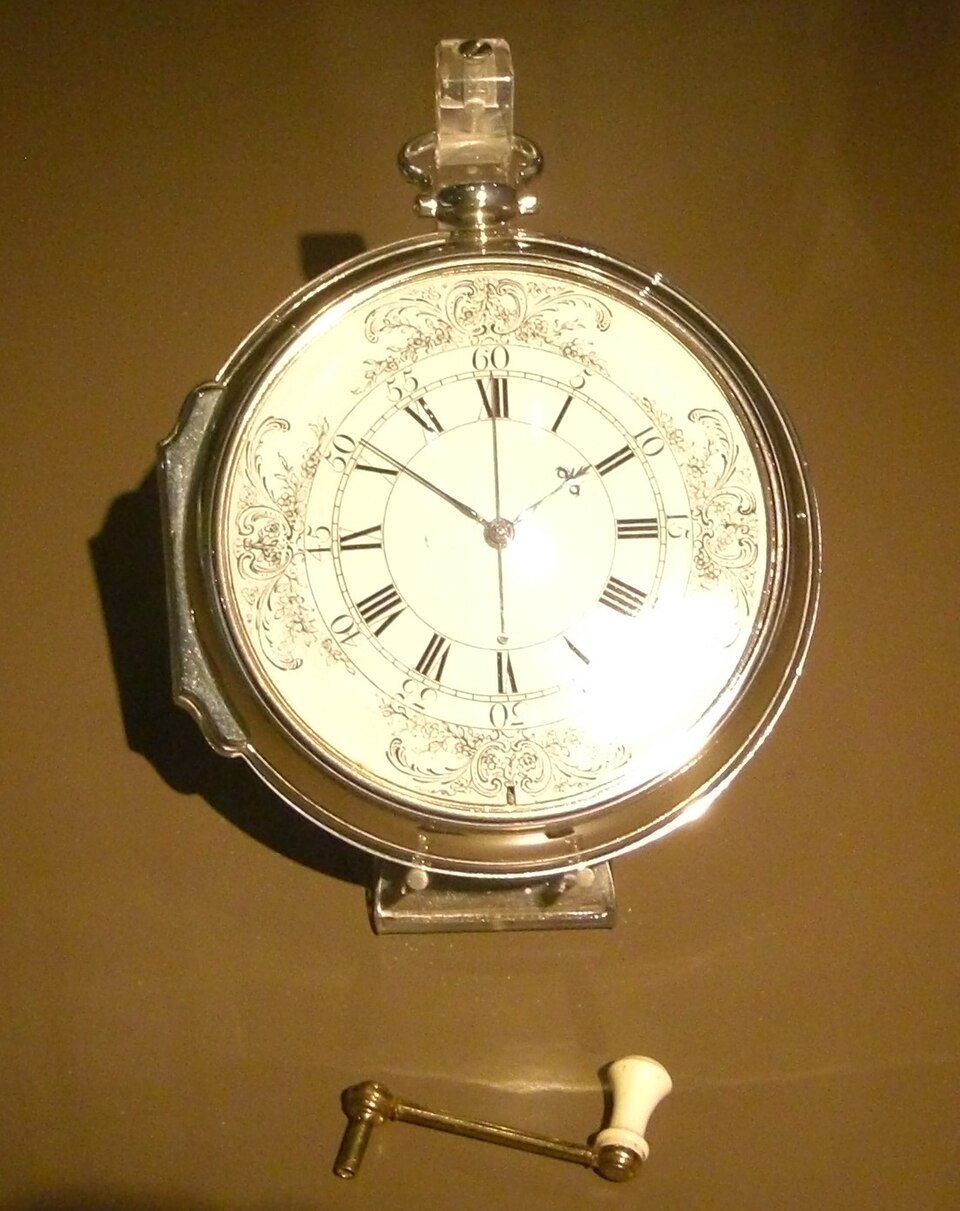
\includegraphics[width=\linewidth]{images/book1/g6-harrison-h4.jpg}\\[2pt]
{\footnotesize 哈里森的 H4，国家海事博物馆，格林尼治。（照片：
Colonel Warden, CC BY-SA 3.0，经维基共享资源。）}
% ledger: commons:harrison-h4
\end{minipage}
\end{history}

\section{练习}

\begin{exercise}[$\star$]\label{exo:g6:latitude-longitude:1}
抄写并补全：“\omterm{def:g6:latitude-longitude:latitude}{纬度}从 \ldots{} 起算，
$0^\circ$ 到 \ldots；\omterm{def:g6:latitude-longitude:longitude}{经度}从 \ldots{} \omterm{def:g6:latitude-longitude:longitude}{经线}起算，取值从
$0^\circ$ 到 \ldots”
\end{exercise}

\begin{exercise}[$\star$]\label{exo:g6:latitude-longitude:2}
\omterm{def:g3:continents-and-oceans:poles}{北极}点的\omterm{def:g6:latitude-longitude:latitude}{纬度}是多少？\omterm{def:g3:continents-and-oceans:poles}{南极}点呢？
\omterm{def:g3:continents-and-oceans:equator}{赤道}上某个城镇的\omterm{def:g6:latitude-longitude:latitude}{纬度}呢？
\end{exercise}

\begin{exercise}[$\star$]\label{exo:g6:latitude-longitude:3}
根据十三座城市的\omterm{def:g2:drawing-to-map:map}{地图}，说明下列每座城市位于\omterm{def:g3:continents-and-oceans:equator}{北半球}
还是\omterm{def:g3:continents-and-oceans:equator}{南半球}，以及在\omterm{def:g6:latitude-longitude:longitude}{本初子午线}的东侧还是西侧，
悉尼、纽约、开罗、里约热内卢。
\end{exercise}

\begin{exercise}[$\star$]\label{exo:g6:latitude-longitude:4}
判断下列说法是否正确，并改正错误的说法。
(a) 所有\omterm{def:g6:latitude-longitude:longitude}{经线}都交于两极。
(b) 所有\omterm{def:g6:latitude-longitude:latitude}{纬线}的长度都相等。
(c) \omterm{def:g3:continents-and-oceans:equator}{赤道}是一条\omterm{def:g6:latitude-longitude:latitude}{纬线}。
(d) \omterm{def:g6:latitude-longitude:longitude}{本初子午线}经过巴黎。
\end{exercise}

\begin{exercise}[$\star\star$]\label{exo:g6:latitude-longitude:5}
根据十三座城市的\omterm{def:g2:drawing-to-map:map}{地图}，哪座城市大约位于
$30^\circ$\,N，$31^\circ$\,E？哪座城市大约位于 $41^\circ$\,N，
$74^\circ$\,W？给出东京的大致坐标。
% ledger: data:b1-ne-places (cities.py main table)
\end{exercise}

\begin{exercise}[$\star\star$]\label{exo:g6:latitude-longitude:6}
城镇 A 位于\omterm{def:g6:latitude-longitude:longitude}{经度} $0^\circ$，城镇 B 位于 $45^\circ$\,E。
两地的正午相差多少小时？哪个城镇先迎来正午？
\end{exercise}

\begin{exercise}[$\star\star$]\label{exo:g6:latitude-longitude:7}
孟买大约位于 $73^\circ$\,E。求其理想\omterm{def:g6:latitude-longitude:time-zone}{时区}。当格林尼治为
正午时，孟买按理想\omterm{def:g6:latitude-longitude:time-zone}{时区}计算是几点？
% ledger: data:b1-ne-places (cities.py: 72.88 E, zone +5)
\end{exercise}

\begin{exercise}[$\star\star$]\label{exo:g6:latitude-longitude:8}
每一度\omterm{def:g6:latitude-longitude:latitude}{纬度}约为 \qty{111}{km}。位于 $30^\circ$\,N 的城镇，
沿所在\omterm{def:g6:latitude-longitude:longitude}{经线}量算，距\omterm{def:g3:continents-and-oceans:equator}{赤道}有多远？\omterm{def:g3:continents-and-oceans:poles}{北极}点距\omterm{def:g3:continents-and-oceans:equator}{赤道}
有多远？
% ledger: rmg:latitude-def
\end{exercise}

\begin{exercise}[$\star\star$]\label{exo:g6:latitude-longitude:9}
纽约位于\omterm{def:g6:latitude-longitude:time-zone}{时区} $-5$，东京位于\omterm{def:g6:latitude-longitude:time-zone}{时区} $+9$。两地的时钟
相差多少小时？纽约为星期一上午 8 点时，
东京是几点、星期几？
% ledger: data:b1-ne-places (cities.py: zones -5 and +9)
\end{exercise}

\begin{exercise}[$\star\star$]\label{exo:g6:latitude-longitude:10}
莉娜说：“太阳从东方升起，所以东边的城镇
会比西边的城镇先看到日出。”她说得对吗？
请结合地球的自转加以解释。
\end{exercise}

\begin{exercise}[$\star\star\star$]\label{exo:g6:latitude-longitude:11}
一艘船上的时钟每天快 3~秒（即走得过快）。(a) 航行
42~天后，时钟快了多少秒？(b) 地球自转 1 度需
4~分钟，即 240~秒。时钟误差会造成多大的\omterm{def:g6:latitude-longitude:longitude}{经度}误差
（以度计）？(c) 在\omterm{def:g3:continents-and-oceans:equator}{赤道}上，\omterm{def:g6:latitude-longitude:longitude}{经度} 1 度约为
\qty{111}{km}。在\omterm{def:g3:continents-and-oceans:equator}{赤道}上，航海者的位置大约偏差
多少千米？
% ledger: rmg:longitude-act-1714, rmg:15deg-per-hour, rmg:latitude-def
\end{exercise}

\begin{exercise}[$\star\star\star$]\label{exo:g6:latitude-longitude:12}
一架飞机于星期一下午 6 点从东京（\omterm{def:g6:latitude-longitude:time-zone}{时区} $+9$）起飞，向东
横越太平洋，飞往洛杉矶（\omterm{def:g6:latitude-longitude:time-zone}{时区} $-8$）。飞行时长为 10~小时。(a)
飞机起飞时，格林尼治的时间是几点？(b) 飞机降落时，
格林尼治的时间是几点？(c) 飞机降落时，洛杉矶
的当地时间和星期几是多少？为何旅客会说，乘坐这趟航班时，“你还没起飞
就已降落了”？
\end{exercise}

\section{问题：环球视频通话}

\begin{problem}[{周末问题——五位朋友、四个时区与一条
日期变更线：视频通话开始时，奥克兰是几点？}]
\label{pb:g6:latitude-longitude:1}
% ledger: data:b1-ne-places, rmg:15deg-per-hour, planet:Earth.day (cities.py, time_zones.py; test_cities_zones_used_in_the_problem)
莉娜住在伦敦。她想和四位度假时结识的朋友组织视频通话。
他们分别是：里约热内卢的安娜、东京的健二、奥克兰的米娅
以及洛杉矶的萨姆。本题采用理想\omterm{def:g6:latitude-longitude:time-zone}{时区}。

\begin{center}
\small
\begin{tabular}{lll}
\hline
朋友 & 城市 & 坐标 \\
\hline
莉娜 & 伦敦 & $52^\circ$\,N, $0^\circ$\\
安娜 & 里约热内卢 & $23^\circ$\,S, $43^\circ$\,W\\
健二 & 东京 & $36^\circ$\,N, $140^\circ$\,E\\
米娅 & 奥克兰 & $37^\circ$\,S, $175^\circ$\,E\\
萨姆 & 洛杉矶 & $34^\circ$\,N, $118^\circ$\,W\\
\hline
\end{tabular}
\end{center}

\medskip
\noindent\textbf{第一部分——朋友们住在哪里。}
\begin{enumerate}
  \item 哪些朋友住在\omterm{def:g3:continents-and-oceans:equator}{南半球}？
  \item 哪些朋友住在\omterm{def:g6:latitude-longitude:longitude}{本初子午线}以西？
  \item 哪位朋友住得离\omterm{def:g3:continents-and-oceans:equator}{赤道}最远？
  \item 哪位朋友住得离 $180^\circ$ \omterm{def:g6:latitude-longitude:longitude}{经线}最近？它与该\omterm{def:g6:latitude-longitude:longitude}{经线}
        相隔多少度\omterm{def:g6:latitude-longitude:longitude}{经度}？
\end{enumerate}

\medskip
\noindent\textbf{第二部分——现在是几点？}
\begin{enumerate}[resume]
  \item 地球每小时自转多少度？
  \item 求出每位朋友所在城市的理想\omterm{def:g6:latitude-longitude:time-zone}{时区}。
  \item 莉娜提议于星期五晚上 8 点（伦敦时间）开始通话。
        此时里约热内卢是什么时间、星期几？东京呢？
  \item 健二回复说，那时他会在睡觉。请解释为什么此时东京已是
        星期六了。
\end{enumerate}

\medskip
\noindent\textbf{第三部分——穿越日期变更线。}
\begin{enumerate}[resume]
  \item 视频通话开始时，洛杉矶是几点、星期几？
  \item 奥克兰的时钟比洛杉矶的快多少小时？
  \item 一艘船从奥克兰向东航行至洛杉矶，途中穿越
        日期变更线。船上日期是前进到次日，还是退回前一日？
  \item 视频通话开始时，奥克兰的当地时间是几点、
        是星期几？
\end{enumerate}
\end{problem}
